\documentclass{article}
\usepackage[utf8]{inputenc}
\usepackage[spanish,mexico]{babel}

\title{Introducci\'on a los Sistemas Complejos\\
\large \quad \\
\large \textbf{An\'alisis de Contagios de COVID-19 en M\'exico (1ra Ola)}
}
\author{Aura De La Garza Garc\'ia\\
311677458}
\date{}
\usepackage{natbib}
\usepackage{graphicx}
\usepackage{amsmath}
\usepackage{amssymb}
\usepackage{amsthm}
\usepackage{enumitem}
\usepackage{mathtools}
\usepackage[a4paper, total={6in, 8in}]{geometry}
\usepackage{pgfplots}
\pgfplotsset{compat=1.18, width=10cm}


\theoremstyle{definition}
\newtheorem{definition}{Ejercicio}

\renewcommand\qedsymbol{$\blacksquare$}

\begin{document}

\maketitle
\section{Introducci\'on}
El siguiente an\'alisis corresponde a la aproximaci\'on de casos diarios de COVID-19 durante la primera mitad del año 2020 (primer Ola), a partir de una curva lognormal. Comenzamos por visualizar nuestros datos a partir de una gr\'afica, en la cual, el eje $x$ corresponde a los d\'ias y el eje $y$ corresponde al n\'umero diario de contagios.

\begin{figure}[htp]
    \centering
    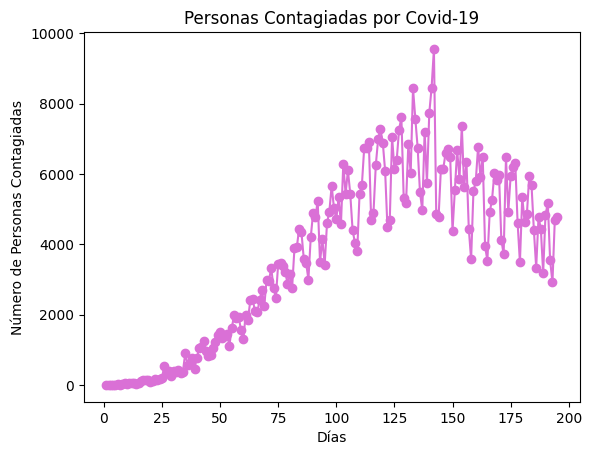
\includegraphics[width=10cm]{covid_casos.png}
    \caption{Datos de COVID-19 (Primera Ola)}
    \label{fig:covdatos}
\end{figure}

Podemos, en efecto notar que, una buena manera de aproximar estos datos es a partir de una curva lognormal. En este caso, utilzaremos una funci\'on lognormal que depende de tres parametros: $A$, $\mu$ y $\sigma$. La raz\'on de utilizar el par\'ametro $A$, se debe a que buscamos una curva que al integrarla no necesariamente nos de como resultado 1, como lo har\'ia una funci\'on de densidad lognormal. Esta funci\'on se escribe de la siguiente manera:
\begin{align*}
    f(x)=A\frac{1}{x}e^{-\frac{(\ln{(x)}-\mu)^2}{2\sigma ^2}}.
\end{align*}

\section{Aproximaci\'on a partir de Algoritmo Gen\'etico}
Para este algoritmo, nuestro programa que aproximar\'a la curva de datos depende de una buena estimaci\'on inicial de los par\'ametros $A$, $\mu$ y $\sigma$. Para ello, haremos una "normaizaci\'on" de nuestros datos, es decir, aplicaremos la funci\'on logaritmo natural al eje $x$, para que nuestra curva de datos se parezca m\'as a una curva normal y podamos encontrar m\'as f\'acilmente una estimaci\'on inicial de datos. 

\begin{figure}[htp]
    \centering
    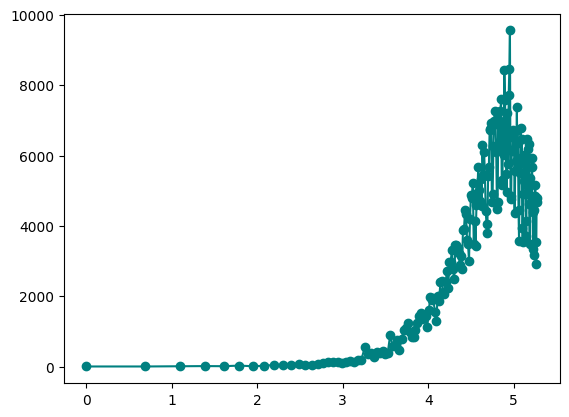
\includegraphics[width=10cm]{datos_norm.png}
    \caption{Normaizaci\'on de Datos}
    \label{fig:datosnorm}
\end{figure}
De acuerdo a la Figura 2, podr\'iamos decir que una buena estimaci\'on incial podr\'ia ser $A_1=8000$, $\mu_1=4.8$ y $\sigma_1=1$. Dados los puntos $(x_1,y_1),(x_2,y_2),\dots,(x_n,y_n)$ correspondientes a los datos de contagios, simularemos incrementos "\textit{aleatorios}" para $A_1$, $\mu_1$ y $\sigma_1$, es decir:
\begin{align*}
    A_2&\mapsto A_1+\Delta A\\
    \mu_2&\mapsto \mu_1+\Delta\mu\\
    \sigma_2&\mapsto \sigma_1+\Delta\sigma.
\end{align*}
Con ello, se calcula
\begin{align*}
    d_1&=\frac{1}{n}\sum_{i=1}^{n}|y_i-f\left(x_i;A_1,\mu_1,\sigma_1\right)|\\
    d_2&=\frac{1}{n}\sum_{i=1}^{n}|y_i-f\left(x_i;A_2,\mu_2,\sigma_2\right)|.
\end{align*}
Si $d_2<d_1$, entonces nuestro programa nos dar\'a $A_2$, $\mu_2$ y $\sigma_2$ como nuevas estimaciones iniciales y se reiniciara el sistema hasta encontrar los par\'ametros \'optimos. Por lo tanto, seg\'un nuestro programa, los par\'ametros \'optimos para la aproximaci\'on con lognormal son los siguientes:
\begin{align*}
    A&=912021.2431162689\\
    \mu&=5.121239439330062\\
    \sigma&=0.4899695205430182.
\end{align*}
A continuaci\'on, podemos observar los datos de contagios diarios junto con la gr\'afica de la funci\'on $f(x;A,\mu,\sigma)$ que mejor aproxima los datos.
\begin{figure}[htp]
    \centering
    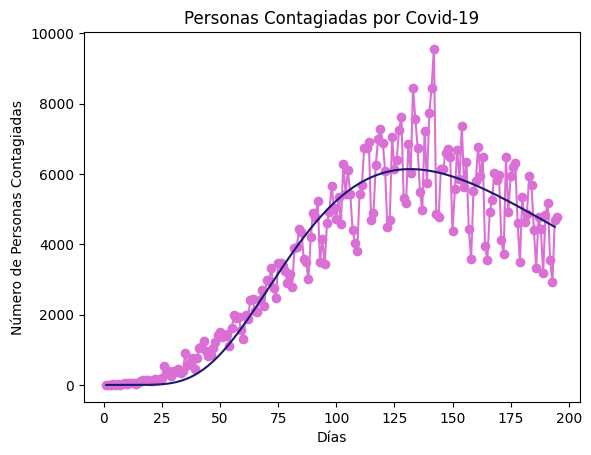
\includegraphics[width=10cm]{covid_y_logn.png}
    \caption{Aproximaci\'on de Datos con lognormal}
    \label{fig:covidlogn}
\end{figure}
\end{document}